\documentclass[12pt,a4paper]{article}

\usepackage[a4paper,text={16.5cm,25.2cm},centering]{geometry}
\usepackage{lmodern}
\usepackage{amssymb,amsmath}
\usepackage{bm}
\usepackage{graphicx}
\usepackage{microtype}
\usepackage{hyperref}
\usepackage{minted}
\setlength{\parindent}{0pt}
\setlength{\parskip}{1.2ex}

\hypersetup
       {   pdfauthor = {  },
           pdftitle={  },
           colorlinks=TRUE,
           linkcolor=black,
           citecolor=blue,
           urlcolor=blue
       }






\begin{document}



\section{Vaja 02 - linearni sistemi}

Reši sistem linearnih enačb

\begin{verbatim}
x + 2y - 7 = 1
2x - y - 3z = 2
x - z = 3
\end{verbatim}
Če želimo sistem rešit z računalnikom moramo sistem spremeniti v matrično obliko. $Ax = b$. Formalno lahko zapišemo rešitev $x = A^{-1} * b$, toda imamo boljše alternative. alternative: reši sistem z LU razcepom. $A = L*U$, kjer L je spodnje trikotna matrika, U pa zgornje trikotna. {\textbackslash} v juliji je operator za deljenje z desne. Torej $A / b = A^{-1} * b$ $b^T / A = b^T * A^{-1}$


\begin{minted}[texcomments = true, mathescape, fontsize=\small, xleftmargin=0.5em]{julia}
A = [1 2 -1; 2 -1 -3; 1 0 -1.0] # matrika sistema

b = [1,2,3] #desne strani

x = A\b # rešitev sistema $A x = b (A / b = A^{-1} b)$
\end{minted}
\begin{minted}[texcomments = true, mathescape, fontsize=\small, xleftmargin=0.5em, frame = leftline]{text}
3-element Vector{Float64}:
  8.000000000000002
 -1.0000000000000002
  5.000000000000001
\end{minted}

Preizkus naredimo tako, da pomnožimo $Ax - b$ enak 0.


\begin{minted}[texcomments = true, mathescape, fontsize=\small, xleftmargin=0.5em]{julia}
A * x - b
\end{minted}
\begin{minted}[texcomments = true, mathescape, fontsize=\small, xleftmargin=0.5em, frame = leftline]{text}
3-element Vector{Float64}:
 8.881784197001252e-16
 0.0
 8.881784197001252e-16
\end{minted}

Sistem lahko rešimo tudi z LU razcepom, tako da sistem $LUx = b$ prevedemo na dva sistema $Ly=b$ in $Ux = y$.


\begin{minted}[texcomments = true, mathescape, fontsize=\small, xleftmargin=0.5em]{julia}
using LinearAlgebra
\end{minted}

p je permutacijski vektor, ki premeša sisteme, tako da optimalno razporedi sisteme za minimiziranje napak.


\begin{minted}[texcomments = true, mathescape, fontsize=\small, xleftmargin=0.5em]{julia}
L,U,p = lu(A)

x = U \ (L \ b[p])
norm(A*x-b, Inf)
\end{minted}
\begin{minted}[texcomments = true, mathescape, fontsize=\small, xleftmargin=0.5em, frame = leftline]{text}
8.881784197001252e-16
\end{minted}

Julia faktorje razcepa zapakira v en objekt.


\begin{minted}[texcomments = true, mathescape, fontsize=\small, xleftmargin=0.5em]{julia}
F = lu(A)
\end{minted}
\begin{minted}[texcomments = true, mathescape, fontsize=\small, xleftmargin=0.5em, frame = leftline]{text}
LinearAlgebra.LU{Float64, Matrix{Float64}, Vector{Int64}}
L factor:
3|$\ensuremath{\times}$|3 Matrix{Float64}:
 1.0  0.0  0.0
 0.5  1.0  0.0
 0.5  0.2  1.0
U factor:
3|$\ensuremath{\times}$|3 Matrix{Float64}:
 2.0  -1.0  -3.0
 0.0   2.5   0.5
 0.0   0.0   0.4
\end{minted}

rezultat je LU, ki je faktorizacija.


\begin{minted}[texcomments = true, mathescape, fontsize=\small, xleftmargin=0.5em]{julia}
x = F \ b
\end{minted}
\begin{minted}[texcomments = true, mathescape, fontsize=\small, xleftmargin=0.5em, frame = leftline]{text}
3-element Vector{Float64}:
  8.000000000000002
 -1.0000000000000002
  5.000000000000001
\end{minted}

\subsection{Tridiagonalne matrike}

\begin{minted}[texcomments = true, mathescape, fontsize=\small, xleftmargin=0.5em]{julia}
using Vaje02
T = Tridiag([1,2],[3,4,5],[6,7])
\end{minted}
\begin{minted}[texcomments = true, mathescape, fontsize=\small, xleftmargin=0.5em, frame = leftline]{text}
Tridiag([1, 2], [3, 4, 5], [6, 7])
\end{minted}

Produkt matrike  z vektorjem 


\begin{minted}[texcomments = true, mathescape, fontsize=\small, xleftmargin=0.5em]{julia}
T * [1,2,3]
\end{minted}
\begin{minted}[texcomments = true, mathescape, fontsize=\small, xleftmargin=0.5em, frame = leftline]{text}
3-element Vector{Int64}:
 15
 30
 19
\end{minted}

Deljenje z leve oziroma operator '{\textbackslash}'


\section{Slučajni sprehod}
\texttt{X\_\{n\} = {\textbackslash}sum\{n,i=1\}Bin(p)} Bin(p) \ensuremath{\tildelow} [[1,-1],[p,1-p]]


\begin{minted}[texcomments = true, mathescape, fontsize=\small, xleftmargin=0.5em]{julia}
"Generator naključnih števil porazdeljenih kot Bin(p)"
rand_bin(p) = (rand() < p) ? 1 : -1
[rand_bin(0.6) for i = 1:10]

sprehod(p,n) = cumsum([rand_bin(p) for i=1:n])

sprehod(0.6,10)

using Plots
scatter(sprehod(0.5,100))
\end{minted}
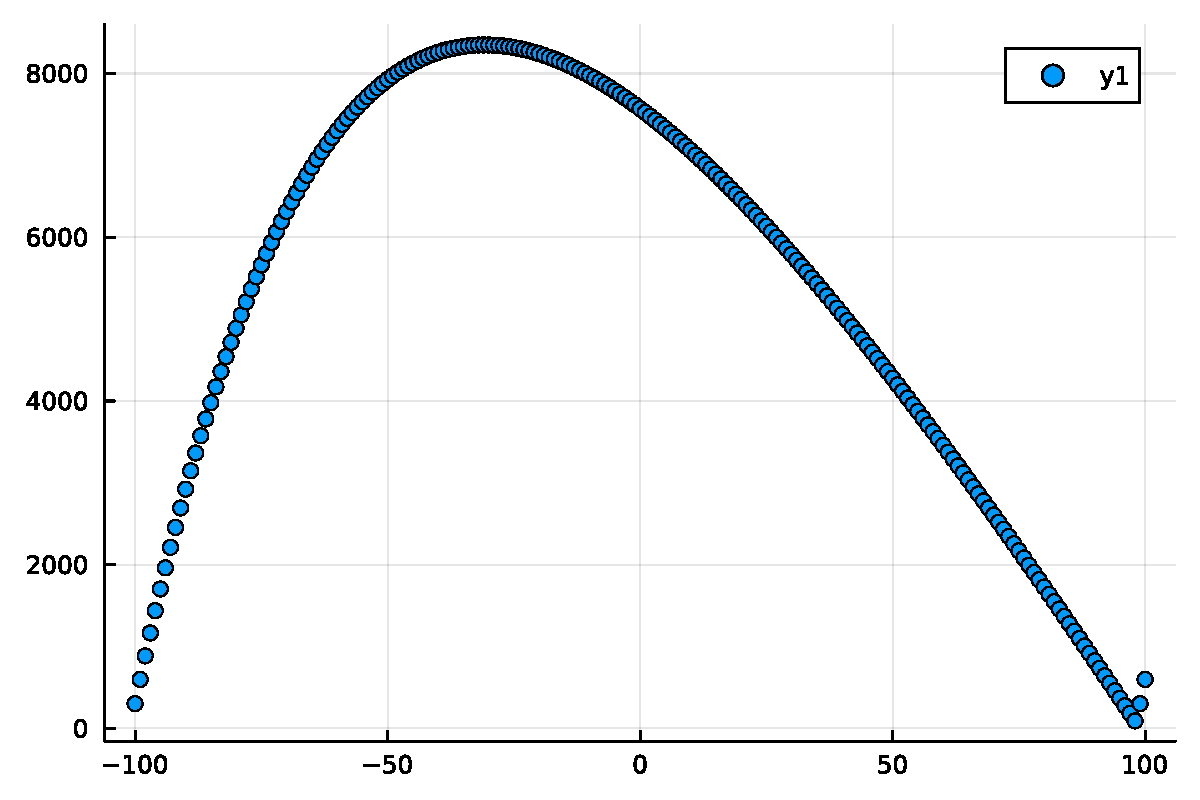
\includegraphics[width=\linewidth]{jl_KF4mRK/demo_9_1.pdf}

\section{Markovske verige $\{X_{n}\}$}
\[
P(X_{n}|X_{n-1}=x_{n-1},X_{n-2}=x_{n-2},...,X_{1}) = x_{1} = P(X_{n-1}) = x_{n-1}
\]

\begin{minted}[texcomments = true, mathescape, fontsize=\small, xleftmargin=0.5em]{julia}
n = 100
p = 0.495
T = Tridiag(-p*ones(2*n-2),ones(2*n-1),-(1-p)*ones(2*n-2))
k = T\ones(2*n-1)
scatter(-n:n,k)
\end{minted}
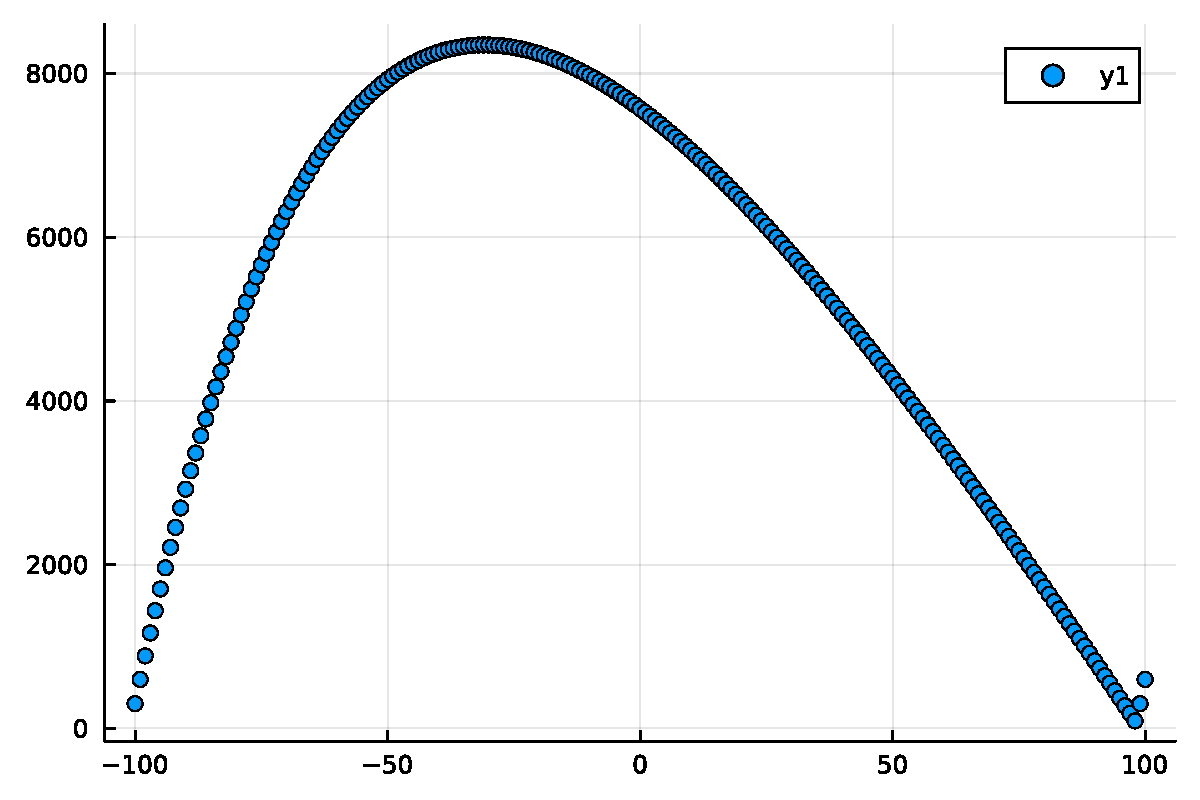
\includegraphics[width=\linewidth]{jl_KF4mRK/demo_9_1.pdf}


\end{document}
